\documentclass[11pt,twoside]{article}
\usepackage{informat}
\usepackage{graphicx}
\graphicspath{{figures/}}

\begin{document}
  \title{Aligning Logical Document Structure with Physical Page Layout}
  \author{Farees Siddiqui and Ken Pu \\
     Faculty of Science, Ontario Tech University \\
     2000 Simcoe Street North, Oshawa, Ontario L1G 0C5, Canada \\
     E-mail: fareesuniversity@gmail.com (TODO: institutional address),
     TODO (K.~Pu)}
  \titleodd{Aligning Logical Document Structure\ldots}
  \authoreven{F. Siddiqui and K. Pu}
  \keywords{document layout analysis, document structure, OCR, alignment, reading order, benchmarking}
  \received{TODO}

  \abstract{A PDF records where glyphs sit on the page but not how the document is
  organised, and the two lines of research that recover that organisation each
  solve half of the problem: structure-oriented OCR produces a hierarchy without
  coordinates, while layout detection produces coordinates without a hierarchy. We
  treat the correspondence between them as a matching problem between two views
  that are produced independently and share neither a tokenisation, nor a
  treatment of mathematics, nor an order of emission. We build both views from the
  same PDF, recover the reading order of the detected regions by recursive XY
  cutting, and compare two aligners resting on opposite assumptions: one
  positional, matching the two sides as character streams, and one order-free,
  matching text embeddings. Both may decline to match, since page furniture
  belongs to no node. We evaluate against an automatic placement procedure at the
  level of words, and against human annotation at the level of whole nodes. The
  first evaluation shows that automatically produced ground truth can fabricate
  the errors it is meant to detect: 2808 of the 3730 misattributions it charged
  against the positional aligner pointed at nodes it had itself failed to place,
  and setting those aside lowered that aligner's measured misattribution rate from
  0.63 to 0.30. The two aligners prove complementary rather than ranked, failing
  on different material. Since our corpus is ten born-digital research papers
  rather than scans, the figures we report compare methods on that corpus rather
  than estimate accuracy in general.}
  % Povzetek: the Slovenian-language summary the journal prints under the
  % English abstract. Published papers by non-Slovenian authors do carry one,
  % and it is short (a single sentence), not a translation of the full abstract.
  % TODO (author): have a Slovenian speaker or the editorial office check this.
  \abstractSi{\v{C}lanek obravnava poravnavo logi\v{c}ne strukture dokumenta s
  podro\v{c}ji na straneh dokumenta PDF, primerja dva pristopa k poravnavi in
  pokaže, da lahko samodejno ustvarjeni referen\v{c}ni podatki ustvarijo prav
  tiste napake, ki naj bi jih merili.}

  \maketitle

\section{Introduction}

Most scientific and technical documents are shared as PDF files, a format that records where glyphs and graphics sit on the page but nothing about how the content is organised. Work on recovering that organisation has split into two mostly separate lines of research. Structure-oriented systems, most recently multimodal models that read a page as an image and emit text~\cite{nougat}, transcribe a document into a hierarchical representation such as Markdown. They capture sections, paragraphs, lists, and formulas, but they lose track of where on the page each element came from. Layout-oriented systems do the opposite: they detect the physical regions of each page (text blocks, tables, figures, headers) as labelled bounding boxes~\cite{publaynet}, but say nothing about how those regions fit together into a document. Neither view is complete on its own. Connecting a node in the logical structure to the pixels that produced it is what makes provenance tracking possible, lets a person visually check OCR output against the original page, and supports interfaces where clicking an element of the document tree highlights it on the page it came from.

This correspondence is harder to establish than it first appears. The two views come from independent models that share no coordinate system, no tokenisation, and no common notion of what counts as a unit. The text of a structural node and the recognised text of a layout region never agree byte for byte, because the two recognisers handle whitespace, hyphenation, ligatures, and mathematics differently; a formula may appear as \LaTeX{} markup on one side and as raw glyphs, or nothing at all, on the other. The mapping is not one-to-one either: a single paragraph node can span several detected regions, across columns or even pages, and a single region can merge material from neighbouring nodes. Layout detectors also report page furniture such as running headers, footers, and page numbers, which has no counterpart in the logical structure and should stay unmatched rather than be forced onto the nearest node. Finally, detectors emit regions in an order that has little to do with how a person reads the page, so in multi-column documents the sequence of regions and the sequence of nodes disagree systematically. Any alignment strategy that assumes the two sides move forward together breaks down at exactly this point. Figure~\ref{fig:concept} shows several of these difficulties on a single page.

\begin{figure*}[t]
  \begin{center}
    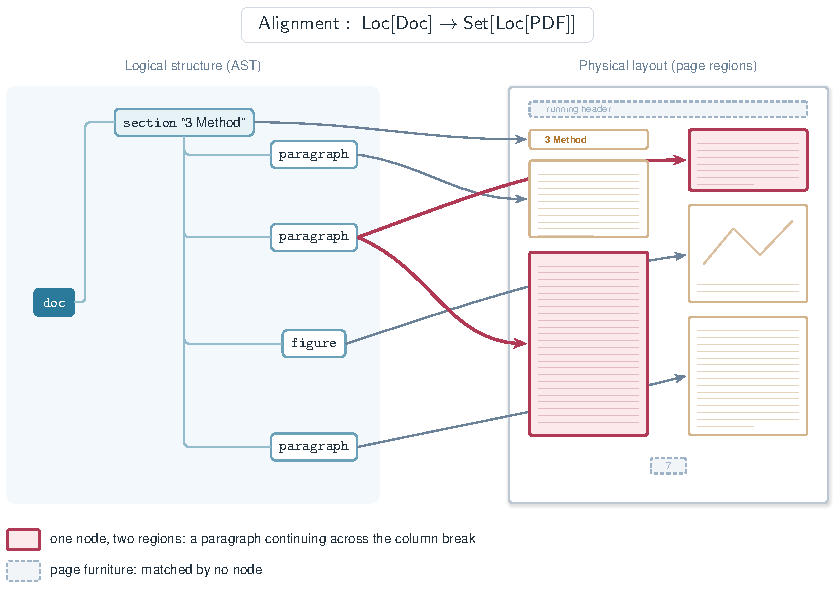
\includegraphics[width=170mm]{fig1_concept}
  \end{center}
  \caption{The two views of a document and the alignment between them. The
  logical structure carries type and hierarchy but no position; the page regions
  carry position but no structure. The mapping is not one-to-one: the second
  paragraph node covers two regions because the paragraph continues across the
  column break, while page furniture such as the running header and the page
  number is matched by no node at all.}
  \label{fig:concept}
\end{figure*}

Correspondences between structure and layout are not themselves new, but they have arrived in two forms, and neither is the one this problem presents. In the first, the correspondence is a means of building datasets: PubLayNet matches PDF pages against the publisher's XML~\cite{publaynet} and DocBank renders the \LaTeX{} source that produced the page~\cite{docbank}, so the structured side is the origin of the PDF and the mapping is guaranteed by provenance. In the second, the logical structure is assembled upward from the detected regions themselves, as in hierarchical structure parsing~\cite{hrdoc} and in conversion toolkits that keep a bounding box on every element they emit~\cite{docling}; there the correspondence holds by construction, and the structure can be no better than the detector beneath it. Our setting is the remaining case, and the ordinary one for a reader holding a published paper: no source is available, and the structure is produced by a recogniser that read the page independently of the detector. The correspondence must then be inferred between two fallible views, which is why matching, the option to abstain, and an evaluation able to distinguish a genuine failure from a disagreement all become necessary. Section~\ref{sec:related} develops these comparisons.

In this paper we study that problem end to end in a working system. Given a PDF, the system builds the two views independently: a large OCR model transcribes the document to Markdown, which we parse into a typed abstract syntax tree (AST) of sections, paragraphs, lists, formulas, and figures, while a separate layout detector finds the physical regions of each page and a text recogniser reads the words inside them. A reading-order module based on recursive XY cutting~\cite{nagy84}, in the refined form proposed by Liu et al.~\cite{xycutpp}, then sorts the detected regions into the order a person would read them, turning an unordered set of regions into a sequence that can be compared with the AST. On top of these two views we implement and compare two aligners built on opposite assumptions. The first is a sequence aligner that concatenates each side into a text stream and matches them character by character, trusting the recovered reading order. The second ignores order entirely and matches nodes to regions by the semantic similarity of their text embeddings. Both are fuzzy by design: a candidate pair below a similarity threshold is left unmatched, since an honest ``no match'' is a valid and necessary outcome.

Measuring how well the two aligners work turned out to be as difficult as building them, because no public dataset pairs the logical structure of a document with the page regions it came from. We therefore evaluate at two levels. The first works at the level of individual words: an automatic placement procedure locates the text of each node in the text layer the PDF already carries, which gives every word on the page an owning node, and the aligner is then scored on whether it attributes each word correctly and whether it abstains where no node applies. Building this benchmark exposed a trap worth reporting on its own. The placement procedure cannot place every node, since formulas surface as markup, figures as image references, and some nodes are too short to locate reliably; treating those nodes as though they owned nothing charges the aligner with an error at exactly the moments it succeeds where the procedure failed. Across our ten documents, of the 3730 misattributions the benchmark charged against the positional aligner, 2808 pointed at a node the procedure had itself been unable to place. Setting those cases aside lowered the measured misattribution rate from 0.63 to 0.30 for that aligner, and from 0.65 to 0.44 for the order-free one. Ground truth produced by an automatic procedure can therefore manufacture the very errors it claims to measure, and the failure is easy to miss because the contaminated numbers are internally consistent and fall in a plausible range.

The second evaluation works at the level of whole nodes against human judgements, collected with an annotation tool written for the purpose. Each node's ground truth records the regions it occupies, or that it appears nowhere, and carries the provenance of that judgement, so that a result resting mostly on unreviewed automatic placement is reported as such instead of being presented as verified. A node counts as correctly located when the area its predicted regions cover overlaps the annotated area by at least half. Under both protocols neither aligner dominates. The positional aligner is the stronger of the two on running prose, while the order-free aligner recovers material the positional one loses wherever the recovered reading order is wrong; the clearest case is tables, although the eight table nodes our annotation currently covers are too few to settle the question. What the two protocols agree on is that the failures are complementary rather than nested, which suggests that the choice between the aligners is a choice of regime rather than of quality.

This paper makes four contributions. First, it treats the correspondence between logical document structure and physical page layout as a matching problem between two independently produced views, rather than as a byproduct of shared provenance, and implements that framing end to end for real documents. Second, it presents two aligners resting on opposite assumptions about order, together with the reading-order recovery that the positional one depends on, and compares them under a single protocol. Third, it contributes two evaluation protocols and the annotation tool behind them, including a node-level localisation benchmark whose ground truth records where each judgement came from. Fourth, it reports two findings about method rather than about magnitude: that automatically produced ground truth can fabricate the errors it is meant to detect, and that order-based and similarity-based alignment fail on different material, so that neither is simply better than the other. We draw this distinction deliberately, because our corpus consists of ten born-digital research papers rather than scans: the accuracy figures we report should be read as a comparison between methods on that corpus and not as a general estimate, whereas the two methodological findings concern how such systems are evaluated and we expect them to hold wherever ground truth is generated automatically.

% TODO (author): confirm before submission whether the implementation, the
% annotation tool and the collected annotations will be released, and add an
% availability statement here if so.

The remainder of the paper reviews related work on document structure recovery, layout analysis and reading order; describes how the two views are built and made comparable; presents the two aligners; sets out the two evaluation protocols and the annotation tool; reports results on our corpus; and discusses what the two findings imply for future evaluation of document alignment.

\section{Related Work}
\label{sec:related}

\textbf{Document structured extraction.} The first line of work converts a document into a structured textual representation. Classical pipelines assembled this from the PDF's own text operators using typographic rules, which is fast but brittle whenever a publisher's visual conventions differ from those the rules encode. Recent systems read the rendered page directly instead. Donut removes the separate OCR stage altogether and maps a document image to structured output with a single encoder-decoder~\cite{donut}; Nougat targets academic papers and emits markup preserving sections, lists, and mathematics~\cite{nougat}; GOT-OCR~2.0 treats formulas, tables, and charts as further classes of ``character'' to be transcribed by one unified model~\cite{gotocr}; and olmOCR distils this capability into models small enough to run over large corpora~\cite{olmocr}. Evaluation of these systems has been fragmented across subtasks, which READoc addresses by scoring the conversion of a multi-page PDF to Markdown as a single end-to-end task~\cite{readoc}. What all of them return is a token sequence in which hierarchy is expressed through markup and the geometry of the page is absent. A reader who asks which pixels produced a given sentence has no way to ask it.

\textbf{Layout analysis.} The second line treats the page as an image and detects its regions. Progress has been driven by datasets: PubLayNet supplies over 360,000 automatically labelled pages from PubMed Central~\cite{publaynet}, DocBank adds token-level labels for 500,000 pages~\cite{docbank}, and DocLayNet contributes 80,863 manually annotated pages chosen for layout variety~\cite{doclaynet}. Detectors range from generic object detectors trained on these corpora to multimodal models such as LayoutLM, which fuses text, position, and image evidence~\cite{layoutlm}, and more recently to unified formulations such as DLAFormer, which casts region detection, logical role classification, and reading order as relation prediction within a single transformer~\cite{dlaformer}. The output is a set of labelled regions with coordinates, precisely what the structure-oriented systems lack. What it does not contain is the document: a region labelled \emph{text} carries no statement about which section contains it, which paragraph it continues, or how it nests. We note that the authors of DocLayNet observe that PubLayNet and DocBank draw exclusively from scientific article repositories and so under-represent layout variety~\cite{doclaynet}; the same caution applies to our own corpus, and we return to it when interpreting our results.

\textbf{Building structure on top of layout.} The gap between the two lines has been attacked directly, and this work is the closest to ours. HRDoc provides 2,500 documents annotated at line level with categories and parent relations, and casts recovery of the logical document as unit classification, parent finding, and relation classification~\cite{hrdoc}. Detect-Order-Construct extends this to a tree-construction pipeline evaluated on Comp-HRDoc, a benchmark spanning region detection, reading order, table-of-contents extraction, and hierarchy in one protocol~\cite{doc}. In parallel, conversion toolkits such as Docling~\cite{docling} and MinerU~\cite{mineru} assemble a structured document in which every element retains its page and bounding box. These systems clearly do deliver both views at once, and it is worth being precise about how our setting differs rather than claiming a gap where none exists. In all of them the logical structure is \emph{defined over} the physical units: a section is a grouping of detected lines or regions, so the correspondence is an artefact of construction and cannot be wrong independently of the detection that produced it. Two consequences follow. The structure can be no better than the detector beneath it, and content the detector misses or misreads, which in our experience means mathematics and material spanning columns, cannot be repaired further up the pipeline. Our setting inverts the dependency. The structure comes from a recogniser that read the page on its own terms and may recover exactly what the detector represents poorly, but the price of that independence is that the correspondence is no longer given and has to be inferred. That inference, and the question of how to evaluate it when it may legitimately return nothing, is the subject of this paper.

\textbf{Reading order.} Detected regions arrive in an order determined by the detector, not by the reader. The classical remedy is the recursive XY cut of Nagy and Seth, which splits a page at horizontal and vertical gaps that no region straddles and recurses on the parts~\cite{nagy84}. Learned approaches treat ordering as a sequence problem: LayoutReader trains a sequence-to-sequence model over text and layout using order harvested from the XML metadata of Word documents~\cite{layoutreader}, and later work recasts the task as the prediction of ordering relations between regions~\cite{orderrel}. XY-Cut++ returns to the geometric formulation and adds pre-masking of high-flexibility elements together with multi-granularity segmentation, repairing the failures the plain recursive cut exhibits on figures and spanning titles~\cite{xycutpp}. Throughout this literature reading order is the end product, valued for feeding retrieval or language-model pipelines with text in a sensible sequence. For us it is a precondition rather than a goal: one of our two aligners depends on it entirely and the other ignores it, which is what allows us to measure what a wrong reading order actually costs.

\textbf{Alignment as supervision.} Where correspondences between structure and layout have been computed, it has usually been to manufacture training data rather than as a task evaluated in its own right. PubLayNet matches pages against publisher XML~\cite{publaynet}, DocBank propagates token colours back from rendered \LaTeX{}~\cite{docbank}, and ReadingBank extracts order from Word metadata~\cite{layoutreader}. The same strategy appears in the historical document literature, where Toselli et al. force-align the text of scholarly digital editions to page images and use the resulting regions as distant supervision for layout analysis of printed books~\cite{toselli}. In every case one side is a privileged source: either the origin of the PDF or an independently produced transcription accepted as correct. Our two views have no such asymmetry, and neither can be taken as the reference against which the other is scored.

\textbf{The reliability of automatic ground truth.} Because these correspondences are produced at a scale that forbids inspection, a large body of ground truth is in circulation that has never been audited. That this matters is not a new observation: Northcutt et al. found label errors averaging at least 3.3\% across ten widely used test sets, and enough of them to change which model a benchmark ranks first~\cite{northcutt}. Their errors are human mistakes scattered through the data. The failure we report is different in kind and, we think, more dangerous, because it is systematic: a placement procedure that cannot handle certain node types produces errors that correlate precisely with the material distinguishing the methods under test, so the bias survives averaging and grows with the size of the corpus. This is what motivates the provenance-tiered ground truth of our second evaluation.

\begin{thebibliography}{99}

  \bibitem{nougat} Blecher, L., Cucurull, G., Scialom, T., Stojnic, R. (2023)
  Nougat: Neural Optical Understanding for Academic Documents,
  {\it arXiv preprint arXiv:2308.13418}.
  DOI: https://doi.org/10.48550/arXiv.2308.13418

  \bibitem{publaynet} Zhong, X., Tang, J., Jimeno Yepes, A. (2019) PubLayNet:
  Largest Dataset Ever for Document Layout Analysis, {\it Proceedings of the 15th
  International Conference on Document Analysis and Recognition (ICDAR)}, IEEE,
  Sydney, pp. 1015--1022.
  DOI: https://doi.org/10.1109/ICDAR.2019.00166

  \bibitem{docbank} Li, M., Xu, Y., Cui, L., Huang, S., Wei, F., Li, Z., Zhou, M.
  (2020) DocBank: A Benchmark Dataset for Document Layout Analysis,
  {\it Proceedings of the 28th International Conference on Computational
  Linguistics (COLING)}, Barcelona, pp. 949--960.
  DOI: https://doi.org/10.18653/v1/2020.coling-main.82

  \bibitem{nagy84} Nagy, G., Seth, S. C. (1984) Hierarchical Representation of
  Optically Scanned Documents, {\it Proceedings of the 7th International
  Conference on Pattern Recognition}, Montreal, pp. 347--349.

  \bibitem{xycutpp} Liu, S., Li, Y., Wei, J. (2025) XY-Cut++: Advanced Layout
  Ordering via Hierarchical Mask Mechanism on a Novel Benchmark,
  {\it arXiv preprint arXiv:2504.10258}.
  DOI: https://doi.org/10.48550/arXiv.2504.10258

  \bibitem{donut} Kim, G., Hong, T., Yim, M., Nam, J., Park, J., Yim, J.,
  Hwang, W., Yun, S., Han, D., Park, S. (2022) OCR-free Document Understanding
  Transformer, {\it Proceedings of the European Conference on Computer Vision
  (ECCV)}, Tel Aviv.
  DOI: https://doi.org/10.48550/arXiv.2111.15664

  \bibitem{doclaynet} Pfitzmann, B., Auer, C., Dolfi, M., Nassar, A. S.,
  Staar, P. W. J. (2022) DocLayNet: A Large Human-Annotated Dataset for
  Document-Layout Analysis, {\it Proceedings of the 28th ACM SIGKDD Conference
  on Knowledge Discovery and Data Mining (KDD)}, Washington DC, pp. 3743--3751.
  DOI: https://doi.org/10.1145/3534678.3539043

  \bibitem{layoutlm} Xu, Y., Li, M., Cui, L., Huang, S., Wei, F., Zhou, M.
  (2020) LayoutLM: Pre-training of Text and Layout for Document Image
  Understanding, {\it Proceedings of the 26th ACM SIGKDD International
  Conference on Knowledge Discovery and Data Mining (KDD)}, pp. 1192--1200.
  DOI: https://doi.org/10.1145/3394486.3403172

  \bibitem{layoutreader} Wang, Z., Xu, Y., Cui, L., Shang, J., Wei, F. (2021)
  LayoutReader: Pre-training of Text and Layout for Reading Order Detection,
  {\it Proceedings of the 2021 Conference on Empirical Methods in Natural
  Language Processing (EMNLP)}, pp. 4735--4744.
  DOI: https://doi.org/10.18653/v1/2021.emnlp-main.389

  \bibitem{gotocr} Wei, H., Liu, C., Chen, J., Wang, J., Kong, L., Xu, Y.,
  Ge, Z., Zhao, L., Sun, J., Peng, Y., Han, C., Zhang, X. (2024) General OCR
  Theory: Towards OCR-2.0 via a Unified End-to-end Model,
  {\it arXiv preprint arXiv:2409.01704}.
  DOI: https://doi.org/10.48550/arXiv.2409.01704

  \bibitem{olmocr} Poznanski, J., Borchardt, J., Dunkelberger, J., Huff, R.,
  Lin, D., Rangapur, A., Wilhelm, C., Lo, K., Soldaini, L. (2025) olmOCR 2:
  Unit Test Rewards for Document OCR, {\it arXiv preprint arXiv:2510.19817}.
  DOI: https://doi.org/10.48550/arXiv.2510.19817

  \bibitem{readoc} Li, Z., Abulaiti, A., Lu, Y., Lin, H., Han, X., Sun, L.
  (2024) READoc: A Unified Benchmark for Realistic Document Structured
  Extraction, {\it arXiv preprint arXiv:2409.05137}.
  DOI: https://doi.org/10.48550/arXiv.2409.05137

  \bibitem{dlaformer} Wang, J., Hu, K., Huo, Q. (2024) DLAFormer: An End-to-End
  Transformer For Document Layout Analysis, {\it Document Analysis and
  Recognition -- ICDAR 2024}, Springer, pp. 40--57.
  DOI: https://doi.org/10.1007/978-3-031-70546-5\_3

  \bibitem{hrdoc} Ma, J., Du, J., Hu, P., Zhang, Z., Zhang, J., Zhu, H.,
  Liu, C. (2023) HRDoc: Dataset and Baseline Method Toward Hierarchical
  Reconstruction of Document Structures, {\it Proceedings of the AAAI Conference
  on Artificial Intelligence}, vol. 37, pp. 1870--1877.
  DOI: https://doi.org/10.48550/arXiv.2303.13839

  \bibitem{doc} Wang, J., Hu, K., Zhong, Z., Sun, L., Huo, Q. (2024)
  Detect-Order-Construct: A Tree Construction based Approach for Hierarchical
  Document Structure Analysis, {\it Pattern Recognition}, Elsevier.
  DOI: https://doi.org/10.48550/arXiv.2401.11874

  \bibitem{docling} Auer, C., Lysak, M., Nassar, A., Dolfi, M., Livathinos, N.,
  Vagenas, P., Ramis, C. B., Omenetti, M., Lindlbauer, F., Dinkla, K., et al.
  (2024) Docling Technical Report, {\it arXiv preprint arXiv:2408.09869}.
  DOI: https://doi.org/10.48550/arXiv.2408.09869

  \bibitem{mineru} Niu, J., Zhang, P., Feng, Z., Li, W., Sun, D., Wang, B.,
  Zhang, B., et al. (2025) MinerU2.5: A Decoupled Vision-Language Model for
  Efficient High-Resolution Document Parsing,
  {\it arXiv preprint arXiv:2509.22186}.
  DOI: https://doi.org/10.48550/arXiv.2509.22186

  \bibitem{orderrel} Xing, C., Wang, R., Nie, Y., Wang, Y., Zhang, M. (2024)
  Modeling Layout Reading Order as Ordering Relations for Visually-rich Document
  Understanding, {\it Proceedings of the 2024 Conference on Empirical Methods in
  Natural Language Processing (EMNLP)}, pp. 9658--9678.
  DOI: https://doi.org/10.18653/v1/2024.emnlp-main.540

  \bibitem{toselli} Toselli, A. H., Wu, S., Smith, D. A. (2021) Digital Editions
  as Distant Supervision for Layout Analysis of Printed Books,
  {\it Document Analysis and Recognition -- ICDAR 2021}, Springer, pp. 462--476.
  DOI: https://doi.org/10.48550/arXiv.2112.12703

  \bibitem{northcutt} Northcutt, C. G., Athalye, A., Mueller, J. (2021)
  Pervasive Label Errors in Test Sets Destabilize Machine Learning Benchmarks,
  {\it Proceedings of the 35th Conference on Neural Information Processing
  Systems (NeurIPS), Track on Datasets and Benchmarks}.
  DOI: https://doi.org/10.48550/arXiv.2103.14749

\end{thebibliography}

\end{document}
